\documentclass[
10pt, % Main document font size
a4paper, % Paper type, use 'letterpaper' for US Letter paper
oneside, % One page layout (no page indentation)
%twoside, % Two page layout (page indentation for binding and different headers)
headinclude,footinclude, % Extra spacing for the header and footer
BCOR5mm, % Binding correction
]{scrartcl}


%----------------------------------------------------------------------------------------
%	REQUIRED PACKAGES
%----------------------------------------------------------------------------------------

\usepackage[
nochapters, % Turn off chapters since this is an article        
beramono, % Use the Bera Mono font for monospaced text (\texttt)
eulermath,% Use the Euler font for mathematics
pdfspacing, % Makes use of pdftex’ letter spacing capabilities via the microtype package
dottedtoc % Dotted lines leading to the page numbers in the table of contents
]{classicthesis} % The layout is based on the Classic Thesis style

\usepackage{arsclassica} % Modifies the Classic Thesis package

\usepackage[T1]{fontenc} % Use 8-bit encoding that has 256 glyphs

\usepackage[utf8]{inputenc} % Required for including letters with accents

\usepackage{graphicx} % Required for including images
\graphicspath{{Figures/}} % Set the default folder for images

\usepackage{enumitem} % Required for manipulating the whitespace between and within lists

\usepackage{lipsum} % Used for inserting dummy 'Lorem ipsum' text into the template

\usepackage{subfig} % Required for creating figures with multiple parts (subfigures)

\usepackage{amsmath,amssymb,amsthm} % For including math equations, theorems, symbols, etc

\usepackage{varioref} % More descriptive referencing

\usepackage[german]{babel}

\usepackage{tabularx}

% listings
\usepackage{listings}

\lstdefinestyle{mStyle}{
    basicstyle=\linespread{1.0}\normalsize\ttfamily,
    keepspaces=false,
    keywordstyle=\color{Fuchsia},
    identifierstyle=\color{MidnightBlue},
    commentstyle=\color{Green},
    stringstyle=\color{Mahogany},
    columns=flexible
}

%----------------------------------------------------------------------------------------
%	THEOREM STYLES
%---------------------------------------------------------------------------------------

\theoremstyle{definition} % Define theorem styles here based on the definition style (used for definitions and examples)
\newtheorem{definition}{Definition}

\theoremstyle{plain} % Define theorem styles here based on the plain style (used for theorems, lemmas, propositions)
\newtheorem{theorem}{Theorem}

\theoremstyle{remark} % Define theorem styles here based on the remark style (used for remarks and notes)

%----------------------------------------------------------------------------------------
%	HYPERLINKS
%---------------------------------------------------------------------------------------

\hypersetup{
%draft, % Uncomment to remove all links (useful for printing in black and white)
colorlinks=true, breaklinks=true, bookmarks=true,bookmarksnumbered,
urlcolor=webbrown, linkcolor=RoyalBlue, citecolor=webgreen, % Link colors
pdftitle={}, % PDF title
pdfauthor={\textcopyright}, % PDF Author
pdfsubject={}, % PDF Subject
pdfkeywords={}, % PDF Keywords
pdfcreator={pdfLaTeX}, % PDF Creator
pdfproducer={LaTeX with hyperref and ClassicThesis} % PDF producer
} % Include the structure.tex file which specified the document structure and layout
\hyphenation{Fortran hy-phen-ation} % Specify custom hyphenation points in words with dashes where you would like hyphenation to occur, or alternatively, don't put any dashes in a word to stop hyphenation altogether


%----------------------------------------------------------------------------------------
%	TITLE AND AUTHOR(S)
%----------------------------------------------------------------------------------------

\title{\normalfont\spacedallcaps{Programmentwurf}} % The article title

\subtitle{Check-Mate} % Uncomment to display a subtitle

\author{\spacedlowsmallcaps{David Schmidt \& Moritz Knapp}} % The article author(s) - author affiliations need to be specified in the AUTHOR AFFILIATIONS block

\date{} % An optional date to appear under the author(s)

%----------------------------------------------------------------------------------------

\begin{document}

%----------------------------------------------------------------------------------------
%	HEADERS
%----------------------------------------------------------------------------------------

\renewcommand{\sectionmark}[1]{\markright{\spacedlowsmallcaps{#1}}} % The header for all pages (oneside) or for even pages (twoside)
%\renewcommand{\subsectionmark}[1]{\markright{\thesubsection~#1}} % Uncomment when using the twoside option - this modifies the header on odd pages
\lehead{\mbox{\llap{\small\thepage\kern1em\color{halfgray} \vline}\color{halfgray}\hspace{0.5em}\rightmark\hfil}} % The header style

\pagestyle{scrheadings} % Enable the headers specified in this block

%----------------------------------------------------------------------------------------
%	TABLE OF CONTENTS & LISTS OF FIGURES AND TABLES
%----------------------------------------------------------------------------------------

\maketitle % Print the title/author/date block

\setcounter{tocdepth}{2} % Set the depth of the table of contents to show sections and subsections only

\tableofcontents % Print the table of contents

\listoffigures % Print the list of figures

\newpage % Start the article content on the second page, remove this if you have a longer abstract that goes onto the second page

\section{Intro}

Da wir, David und Moritz, schon immer gerne Schach gegeneinander spielten um auch in Lernpausen unseren Geist nicht zu unterfordern, entschieden wir uns ein eigenes Schach zu programmieren. 
Zudem sind wir davon überzeugt, dass Schach eine perfekte Grundlage für objektorientiertes Programmieren bietet, aufgrund der vielen Figuren die jeweils gerade und schräge Züge individuell ausführen.

\section{Clean-Architecture} \label{sec:cleanArc}
Bereits vor dem Studium hat David schonmal ein Schach programmiert. Dabei handelte es sich um ca 3000 Zeilen hochineffizienten Arduino Code. In diesem Projrekt wollten wir unseren früheren Ichs beweisen wie viel eleganter so etwas umsetzbar ist. Der erste Schritt dazu ist die Clean-Architecture.

\begin{figure}[h]
	\begin{center}
		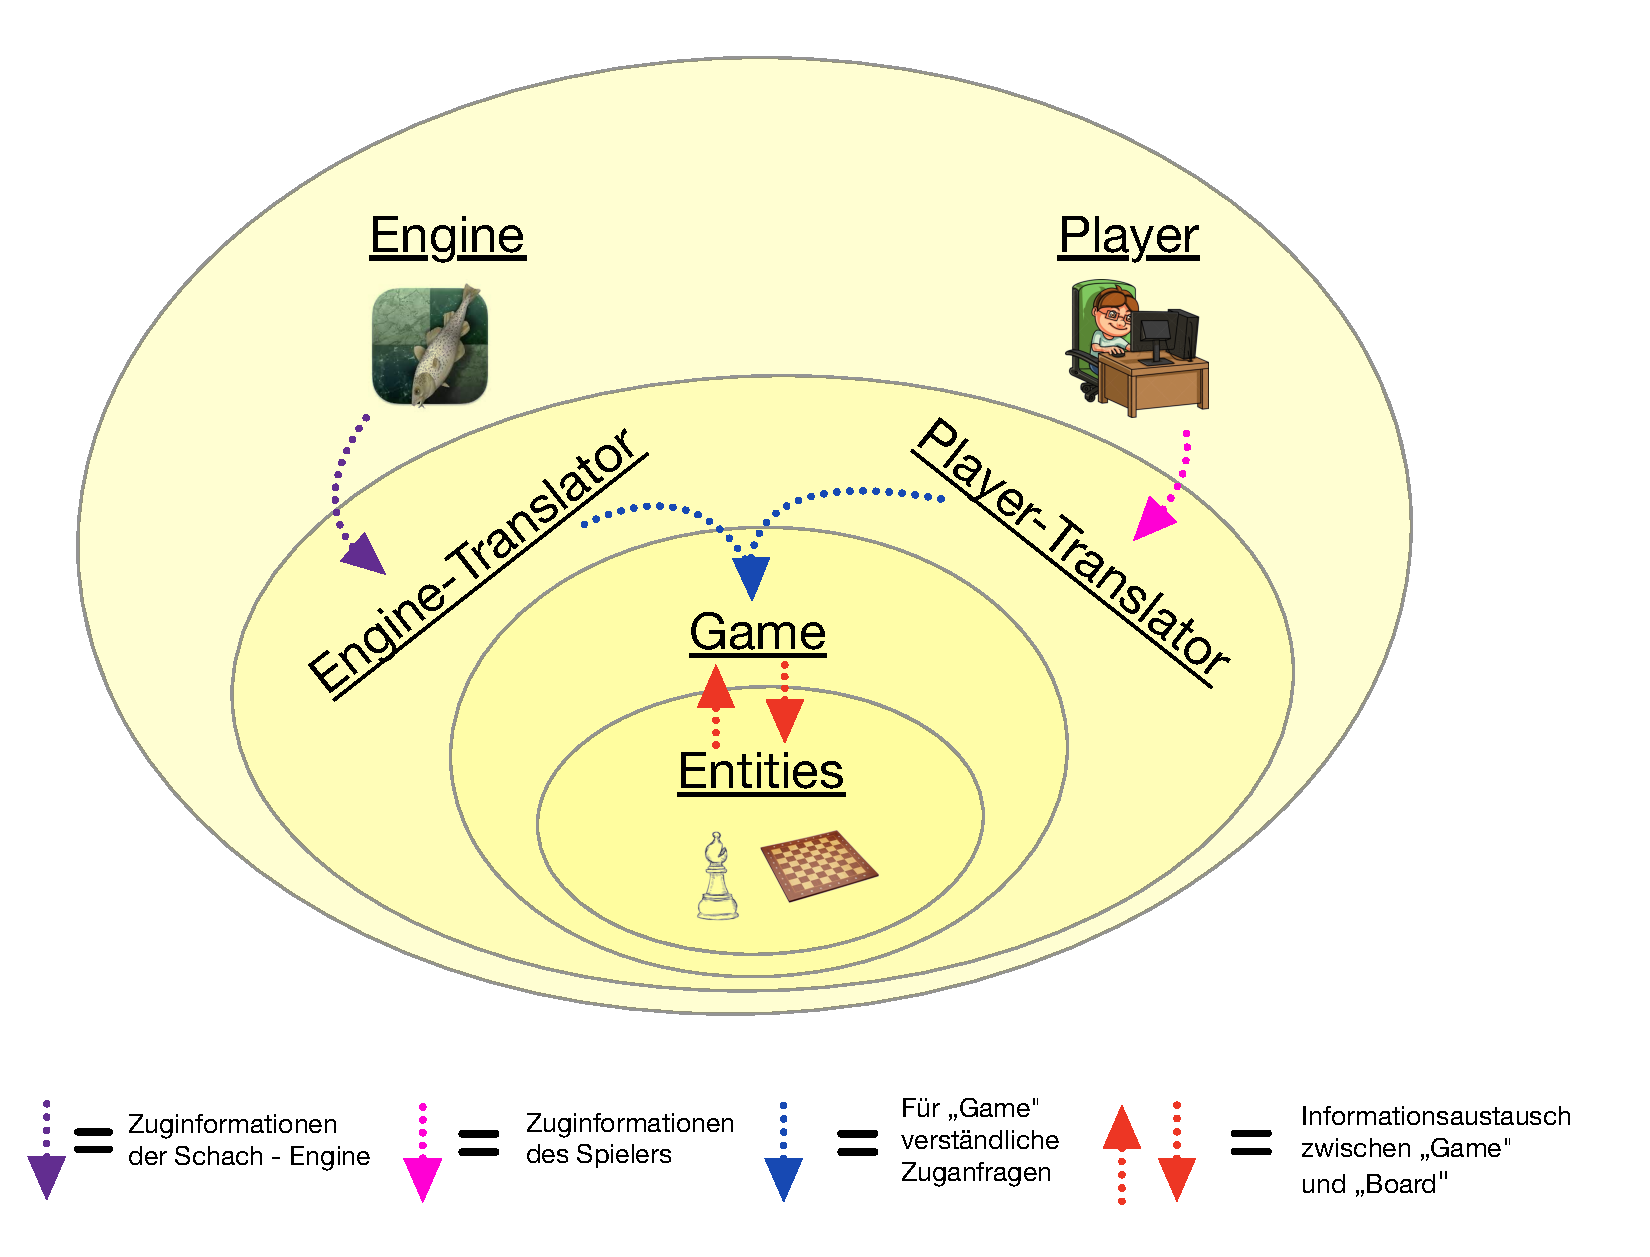
\includegraphics[width = \textwidth]{onion.pdf}
		\caption{Übersicht über die Clean Architecture}
		\label{fig:umlEntities}
	\end{center}
\end{figure}

Zusammengefasst ermöglicht eine Clean Architecture die Veränderung der Umgebung, bzw. des Systems, ohne den eigentlichen Kern des Codes anpassen zu müssen.
Das bedeutet, dass wir theoretisch unser Spiel um ein echtes Spielbrett mit LEDs und Arduino- Raspberry-Steuerung erweitern könnten, ohne unseren Schach-Code zu verädnern.
\newpage
\subsection{Schicht 1: Entities}
Die Entities sind der Kern unseres Spiels. Unabhängig von der Umgebung sind die einzelnen Figuren virtuell auf einem Feld positioniert und können umplatziert werden.
Dadurch ergeben sich grundlegend Folgende Klassen: 

\begin{center}
	\begin{itemize}
		\item Board
		\item Square
		\item Piece
	\end{itemize}
\end{center}

Ein Board besteht aus vielen Squares, auf denen jeweils ein Piece stehen kann. Um dies zu implementieren und später auch verschiedene Pieces zu benutzen, zeigt \autoref{fig:umlEntities} alle Klassen welche unser Kern der Clean-Architektur beinhalten soll. 
\begin{figure}[h]
	\begin{center}
		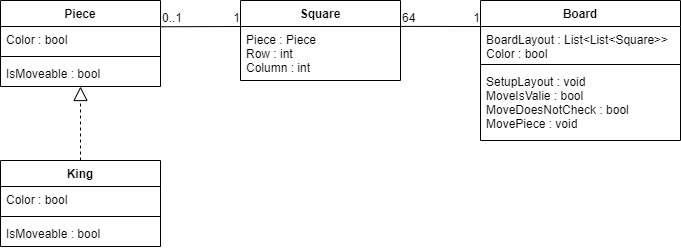
\includegraphics[width=10cm]{entities.png}
		\caption{\label{pic:umlEntities} UML-Diagramm der Entities}
	\end{center}
\end{figure}
Das Diagramm zeigt die Schach-Logik im Kern unserer Clean Architecture, bzw. die Entities. Das \texttt{Board} stellt das Schachbrett dar. Dieses besteht aus 64 \texttt{Squares}. Die Methode \texttt{SetupLayout} erstellt das Board und besetzt die richtigen Felder mit Pieces mit der entsprechenden Farbe.
Von den eigentlichen \texttt{Pieces} ist hier nur der König gezeigt, da die anderen Figuren genau wie er die Methode \texttt{IsMoveable} implementieren. 
Das Board bietet drei Methoden, von denen nur eine tatsächlich von weiteren Schichten verwendet wird: \texttt{MovePiece}. Die Methode überprüft mit \texttt{MoveIsVali} ob es sich um einen Validen Zug handelt. \texttt{MoveIsValid} ruft dabei die von Figuren implementierte Methode \texttt{IsMoveable} auf um zu überprüfen ob die Figur theoretisch in der Lage wäre den Zug durchzuführen.\\ Der wesentliche Unterschied zwischen \texttt{MoveIsValid} und \texttt{IsMoveable} besteht darin, dass Figuren das Board nicht kennen und auch nicht wissen wo sie sich befinden. \texttt{IsMoveable} signalisiert lediglich, ob ein Zug rein von den allgemeinen Zugmöglichkeiten der Figur möglich ist (zB. Läufer kann nur schräg laufen). \texttt{MoveIsValid} ist eine Methode des Boards und kann somit auch situationsbedingte Auskunft über die Validität des Zuges geben. Wenn die Figur \texttt{IsMoveable} ist, wird von \texttt{MoveIsValid} noch überprüft ob weitere Figuren im Weg stehen und der Zug sich selbst in Schach setzen würde (\texttt{MoveDoesNotCheck}). Ist alles überprüft, wird der Zug durchgeführt.

\subsection{Schicht 2: Use-Case}
Die Use-Cases bilden die zweite Schicht der Clean Architekture. Sie können informationen der ersten Schicht erhalten (Entities), diese sind aber nicht abhängig von den Use-Cases.\\
In unserem Fall haben wir nur einen Use-Case: Das Spiel, bzw. \texttt{Game}. Diese Klasse erstellt das Board, bzw ruft die Funktion \texttt{SetupLayout} auf, hat aber noch weitere Informationen die über das einfache Ziehen von Figuren hinausgehen:
\begin{center}
	\begin{itemize}
		\item Spielerposition (z.B. Spieler 1 spielt unten),
		\item Spielerfarbe (z.B. Spieler 1 ist weiß)
		\item und aktueller Spieler (z.B. Spieler 1 ist dran).
	\end{itemize}
\end{center}
Der Use-Case initialisiert das Board, wodurch die Farbe des unten spielenden Spielers zufällig gewählt wird. Logisch betrachtet spielt für das \texttt{Game} Spieler 1 in jedem Fall \textit{unten}. Da immer weiß beginnt, ist es zufällig ob Spieler 1 beginnen darf oder nicht. Welche Art von User-Interface nun Spieler 1 steuert, ist Aufgabe der dritten Schicht, welche in unserem Fall den Menschen an der Gui Spieler 1 und eine Schach-Engine Spieler 2 zuordnet. \texttt{Game} ist von dieser Information jedoch abgekapselt, da eine Zuganfrage in jedem Fall gleich aussieht.
So eine Anfrage ist von \texttt{Game} definiert (z.B. 'e5,e6' = ''Zug von e5 nach e6''). \\
Wird nun eine solche Anfrage gestellt, verlangt \texttt{Game} von \texttt{Board} eine Auskunft über die Farbe der Figur, welche sich auf dem \textit{von}-Feld befindet. Stimmt diese mit der Farbe des aktuell spielenden Spielers überein, kann der Zug nach Validitätsprüfung ausgeführt werden. Anhand dessen ob \texttt{MovePiece} \texttt{true} oder \texttt{false} zurückgibt, ist der andere Spieler daraufhin am Zug, oder nicht.
\subsection{Schicht 3: Übersetzer}
Sollte es dazu kommen, dass die Umgebung beispielsweise zu einer Ascii-Oberfläche geändert wird, müssen ab dieser Schicht Veränderungen am Code erfolgen. Solange jedoch die Zug-Anfragen richtig gestellt werden, arbeitet der Code in den unteren Schichten immer gleich. In der 3. Schicht befindet sich ein GUI- und Engine-Translator. Diese übersetzen Züge von Spieler und Engine und geben sie für diese lesbar codiert an die zweite Schicht. 
Solche Zug-Anfragen können völlig asynchron erfolgen, sie führen jedoch zu nichts, falls der Zug nicht den Regeln entspricht, oder der Spielende nicht am Zug ist.
\subsection{Schicht 4: User-Interfaces}
Auf dieser Ebene befinden sich die Interfaces für die Spieler. In unserem Fall sind das die GUI und die Schachengine. Die GUI wurde mit WPF gebaut. Dieses stellt mithilfe eines Databindigs auf ein Viewmodel des Board-Layouts immer den aktuellen Stand des Spiels grafisch dar. 
Die GUI bietet die Möglichkeit, mithilfe von Mausklicks Figuren zu ziehen (z.B. erster Klick auf \textit{E2}, zweiter Klick auf \textit{E3}~~ $\Rightarrow$ \textit{E2 nach E3}). Diese Klicks werden dann an den PlayerTranslator in Schicht 3 weitergegeben, welcher diese dann in eine für das Game verständliche Anweisungen übersetzt.

Die Einbindung der Engine funktioniert ähnlich, nämlich über einen EngineTranslator, der die Schnittstelle zwischen Game und der Engine ist. Der größte Unterschied ist hier, dass die Engine eine externe Kommandozeilenanwendung ist und daher erst einmal in unsere C\#-Anwendung eingebunden werden muss.
Hierfür wird eine Instanz einer Engine-Klasse erstellt, welche den tatsächlichen Engine-Pozess startet und sich um sämtliche Kommunikation zwischen dem Engine-Prozess und dem EngineTranslator kümmert. Vom EngineTranslator wird hier regelmäßig das aktuelle Layout des Boards abgefragt. Dieses wird dann an die Engine weitergeleitet, welche daraufhin den nächsten besten Zug berechnet. Dieser berechnete Zug wird dann an den Translator zurückgegeben, welcher diesen dann übersetzt und an das Spiel weitergibt.
\section{Programmierprinzipien}
\subsection{pros/cons/wieso wir?}
\subsection{SOLID}
\subsubsection{Single Resposibility Principle}

\subsubsection{Open/Closed Principle}
\colorbox{yellow}{Engine eine liste von commands abarbeiten lassen anstatt Anfragen zu hardcoden}
\subsubsection{Liskov' Substitution Principle}
Piece -> Queen
\subsubsection{Interface Segregation Principle}
\colorbox{yellow}{Interface wo?}
\subsubsection{Dependency Inversion Principle}
Bei Translator wird game eingesetzt statt game direkt zu übergeben. Methoden werden dann auf Translator angewendet.
\subsection{GRASP}
\subsubsection{Low Coupling}
Translator: Game kennt Engine und Player nicht mehr, interessiert sich nur an befehlen.
\subsubsection{High Cohesion}
\colorbox{yellow}{Player auslagern mit eigener Setcolor funktion usw. (Playername??)}

\subsection{DRY (Don't Repeat Yourself)}
Schon umgesetzt?


\section{Unit Testing}
\subsection{pros/cons/wieso wir?}
Tests sind eine der grundlegenden Elemente einer jeder Software-Anwendung. Ohne sie kann der korrekte Ablauf der Anwendung nicht \dots getestet werden. Unit tests verwenden wir in unserem Projekt hauptsächlich dort, wo Berechnungen auf dem Brett durgeführt werden. Diese sind nämlich erfahrungsgemäß sehr fehleranfällig, besonders für die Art von Fehlern, die sich erst durch das Erweitern einer ursprünglichen Funktion einschleichen, entstehen hier sehr schnell. So ist es zum Beispiel gut möglich dass die Bewegungen des Bauerns perfekt regelkonform umgesetzt werden, jedoch nach der zusätzlichen Einführung der \enquote{En passant}-Schlagmöglichkeit plötzlich viele Züge wieder ausführbar sind, die gar nicht erlaubt sein sollten.

Für unser Projekt nutzen wir das XUnit testing Framework, welches uns ermöglicht, ohne viel Aufwand Unit Tests zu erstellen.
XUnit tests sind nach dem folgenden Schema aufgebaut:
\begin{lstlisting}[language=c, style=mStyle]
public class TestClass{
	[Fact]
	public void TestUnit_NoDataPassed()
	{
		// Given
		bool b = false;

		// When
		b.Set(true);

		// Then
		Assert.True(b);
	}

	[Theory]
	[InlineData(1)]
	public void TestUnit_IntPassed(int input)
	{
		//Given
		int val;

		//When
		val = input;

		//Then
		Assert.Equal(1, val);
	}
}
\end{lstlisting}

Eine Testklasse wird verwendet, um zusammengehörende Unit Tests zu verpacken. Jeder Unit Test ist entweder mit \texttt{[Fact]} oder mit \texttt{Theory} annotiert. Das letztere wird verwendet, um zusätzliche externe Daten an den Test zu übergeben. Diese werden dann mit der \texttt{[InlineData]}-Annotation definiert und dann vor dem Test automatisch als Funktionsparameter übergeben.
\subsection{ATRIP}
Für das Entwickeln von guten Unit Tests gelten die ATRIP-Regeln, welche in den folgenden unterkapiteln aufgelistet werden.
\subsubsection{Automatic}
Gute Tests sollen automatisch, bedeutet ohne weiteres eingreifen des Entwicklers, ablaufen. Dazu gehört, dass die Tests regelmäßig automatisch gestartet werden und ihre Ergebnisse danach auch selbstständig überprüfen. Jeder Unit Test sollte nach Ablauf eines der beiden Ergebnisse \enquote{bestanden} und \enquote{nicht bestanden} zurückgeben.
An dieses Prinzip haben wir uns in sämtlichen Unit Test gehalten. Unsere Tests sind nach dem AAA(Arrange, Act, Assert)-Schema aufgebaut, bauen also zu Beginn die nötigen Abhängigkeiten auf, nehmen dann Einfluss auf diese und führen anschließend eine einzige Methode der xUnit.Assert-Klasse aus, um die Korrektheit des Endzustands zu prüfen. Unsere IDE Microsoft VisualStudio haben wir so konfiguriert, dass sämtliche Unit Tests jedes mal automatisch ausgeführt werden, nachdem der Build-Step des Projekts durchgelaufen ist.

\subsubsection{Thorough}
\colorbox{yellow}{Todo wenn alle Tests geschrieben sind}
\subsubsection{Repeatable}
Unit Tests sollten wiederholbar sein, was bedeutet, dass sie nicht auf veränderlichen Daten aufbauen sollten. Solche veränderlichen Daten sind beispielsweise Zufallszahlen, die aktuelle Uhrzeit oder die Anzahl von Dateien im Projektordner. Diese Art von Daten haben wir natürlich konsequent vermieden.
\subsubsection{Independent}
Die Kernaussage von independent Tests ist, dass die Ergebnisse oder die Funktion der Tests nicht abhängig von ihrer Reihenfolge oder Zusammenstellung sein dürfen. Jeder Test sollte vollständig unabhängig von allen anderen Tests sein. Dies haben wir erreicht, indem keine Ressource, die in einem Test verwendet wird, außerhalb dieses Tests weiterbesteht. Stattdessen wird jede Ressource, die ein Test benötigt in seiner Arrange-Phase erstellt und begrenzt sich damit auf den Scope des Tests.
\subsubsection{Professional}
Professionelle Unit Tests sind so einfach verständlich wie möglich gestaltet. Damit soll vermieden werden, das sich Fehler in den Test-Code einschleichen, da diese besonders schwierig und damit besonders teuer zu finden und beheben sind.
Unsere Unit Tests sind klein und überschaubar. Zudem ist unsere Namensgebung so gewählt, dass alle informationen über einen Test durch das Lesen seines Namens erhältlich sind. Ein Beispiel hierfür ist der folgende Unit Test:
\begin{lstlisting}[language=c, style=mStyle]
	[Fact]
	public void GetSquareFromCoords_ReturnedSquare_IsEmpty()
	{
		// Given
		BoardLayout layout = new();

		// When
		layout.SetToStartLayout(new Player());
		
		// Then
		Assert.Null(layout.GetSquareFromCoords(3, 3).Piece);
	}
\end{lstlisting}

\subsection{Code Coverage}
\colorbox{yellow}{TODO}
\subsection{Mocking}
\newpage
\section{Refactoring}
\subsection{Codesmell: Long Method und Switch-case}
Einer früheren Version des Codes war eine Methode zu entnehmen, welche gleich zwei übel riechende Codesmells aufwies. Zum einen war die Methode sehr lang, zum anderen streckte sich ein großes Switch-Case über die gesamte länge. Die Rede ist von jener Methode, welche festetellen soll ob ein Zug valide ist oder nicht. Die Validierung eines Zuges von einem Startfeld zu einem Zielfeld muss die folgenden Voraussetzungen erfüllen:
\begin{center}
	\begin{itemize}
		\item 1. Ist das Zielfeld ein anderes als das Startfeld?
		\item 2. Steht auf dem Startfeld eine Figur?
		\item 3. Kann die Figur tatsächlich so ziehen?
		\item 4. Würde der Zug das eigene Team in Schach setzen?
		\item 5. Darf der Zug so ausgeführt werden (d.h. es sind keine Figuren im Weg und am Ziel befindet sich keine Figur der eigenen Mannschaft)?
	\end{itemize}
\end{center}
Liefert eine dieser Fragen als Ergebnis \texttt{false} wird der Zug als nicht valide gewertet. Wie bereits unter Clean-Architecture erwähnt, kann das Board situationsbedingt Aussagen treffen, die Figur nur Aussagen über die theoretische Ausführung des Zuges. Dadurch ergab sich, dass die theoretische Ausführung eines Zuges polymorph gelöst und die situationsbedingt innerhalb der MoveIsValid-Methode evaluiert wurde. In folgendem Code-Ausschnitt ist zu sehen, wie unter \texttt{movingPiece.IsMoveable(from, to)} die Polymorphe Validierung erfolgt, wonach das große Switch-Case gestartet wird. Hierbei ist nur ein kleiner Teil der Validierung für den Fall einer Dame aufgeführt, um die Größe  und insbesondere den hohen Einrückgrad der Methode zu betonen. 

\begin{lstlisting}[language=c, style=mStyle]
public bool MoveIsValid(Square from, Square to)
{
 if (from.Row == to.Row && from.Column == to.Column) { return false; }
  if (layout.GetAsList()[from.Row][from.Column] != null)
  {
   Piece movingPiece = layout.GetAsList()[from.Row][from.Column].Piece;
   Piece destinationPiece = layout.GetAsList()[to.Row][to.Column].Piece;
   bool movingPieceColor = movingPiece.Color;
   if (movingPiece.IsMoveable(from, to) && MoveDoesNotCheck(from, to))
   {
	if (!movingPiece.MoveIsValid(from, to)) { return false; }
	switch (movingPiece)
	{
	 case Queen:
	  if (destinationPiece?.Color != movingPieceColor)
	  {
	   int rowDifference = Math.Abs(to.Row - from.Row);
	   int columnDifference = Math.Abs(to.Column - from.Column);

	    if (rowDifference == 0)
		{
		 if (to.Column > from.Column)
		 {
		  for (int i = from.Column + 1; i < to.Column; i++)
		  {
		   if (layout.GetAsList()[from.Row][i].Piece != null) { return false; }
		  
\end{lstlisting}

Das Switch-Case über den Instanztyp der Figur soll nun ebenfalls durch einen Polymorphen Methodenaufruf eleminiert werden. 

\subsection{Refactoring: Replace Conditional with Polymorphism}
Das Problem bei einem polymorphen Methodenaufruf hierbei ist, dass die Figur selbst keine Ahnung hat wo sich andere Figuren befinden. Diese Information ist dem Board vorbehalten. Eine Simple Lösung wäre sicherlich, das Board jeder Figur als Übergabeparameter zu geben, dabei geht jedoch die Sinnhaftigkeit der Logik verloren. Dependency Injection schafft heirbei Abhilfe. Es wird ermöglicht, von den Figuren aus Infos über einzelne Felder zu erfragen. Anstatt dass das Board für jedes, sich auf einem Zugpfad befindendes, Feld überprüft ob eine Figur im Weg steht, soll nun die Figur für jedes Feld erfragen, ob eine andere im Weg steht. Die Figur hat also keine Informationen über das Board, sondern nur einen Weg essenzielle Informationen zu erfragen. Umgesetzt wird dies durch ein Interface. Das \texttt{Boardlayout} erbt und implementiert die beiden Methoden \texttt{GetSquare} und \texttt{GetPiece} des Interfaces \texttt{IBoardLayout}. Wie der Namensgebung zu entnehmen ist, geben die Methoden ein Piece oder Square zurück. EInzelne Figuren benötigen nun ein Objekt von \texttt{IBoardLayout}, welches im Konstruktor übergeben wird. Erzeugt nun das BoardLayout eine Dame, muss ein Verweis auf ein \texttt{IBoardLayout} übergeben werden. Eine Erzeugung sieht wie folgt aus:

\begin{lstlisting}[language=c, style=mStyle]
startLayout[0][0].Piece = new Queen(player.Color, this);
\end{lstlisting}

der Parameter \texttt{this} verweist auf das BoardLayout, welches vom Interface \texttt{IBoardLayout} erbt. Im Konstruktor von Queen muss dieses einem lokalen \texttt{IBoardLayout} zugeteilt werden. Daraufhin kann über diese lokale Variable beispielsweise mit \texttt{variable.GetPiece(Square)} das Piece welches sich im BoardLayout auf dem benannten Square befindet abgerufen werden, ohne dass die Dame weitgehende Informationen über das Board besitzt.\\
Infolge dessen implementiert nun jede Figur die Methode \texttt{<bool>MoveIsValid(<Square> from, <Square> to)}. Im folgenden ist die Implementierung von \texttt{MoveIsValid} des Königs gezeigt.

\begin{lstlisting}[language=c, style=mStyle]
public override bool MoveIsValid(Square from, Square to)
{
	return board.GetPiece(to)?.Color != board.GetPiece(from).Color;
}
\end{lstlisting}

\texttt{board} ist die Instanz von \texttt{IBoardLayout}. Dabei wird überprüft, ob sich auf dem Zielfeld eine Figur des eigenen Teams befindet. ist dies der Fall, darf der Zug nicht ausgeführt werden.\\
Innerhalb der Board-Klasse wird nun das riesige Switchcase durch den einfachen Methodenaufruf \texttt{movingPiece.MoveIsValid(from, to);} ersetzt.

\subsection{Refactoring: Replace Temp with Query}
Innerhalb der neuen Methode \texttt{MoveIsValid} kann nun ein weiteres Refactoring angewendet werden. Infolgendem Listing ist die ganze Methode gezeigt.

\begin{lstlisting}[language=c, style=mStyle]
public bool MoveIsValid(Square from, Square to)
{
if (from.Row == to.Row && from.Column == to.Column) { return false; }
if (layout.GetAsList()[from.Row][from.Column] != null)
{
	Piece movingPiece = layout.GetAsList()[from.Row][from.Column]?.Piece;
	if (movingPiece == null) { return false; }

	if (movingPiece.IsMoveable(from, to) && MoveDoesNotCheck(from, to)) //hehe, codesmell
	{
		return movingPiece.MoveIsValid(from, to); //this is the way!!!                    
	}
}
return false;
}
\end{lstlisting}
Zu erkennen ist hierbei die oft genutzte lokale Variable \texttt{movingPiece}. Sie bezeichnet jene Figur, die den zu evaluierenden Zug ausführt. Das hier aufgeführte Refactoring soll die lokale Variable in eine Funktion auslagern, da ein lokaler Cache performancetechnisch ineffizienter ist. Die neue Methode \texttt{getPieceFrom(Square)} gibt die Figur zurück, welche sich auf dem angegebenen Square befindet. Die neue Methode \texttt{MoveIsValid} ohne lokale Variable ist in der Datei Board.cs ab Zeile 25 zu sehen.
\section{Entwurfsmuster}
\subsection{Diagramme und Begründungen}

\section{Fazit}\label{sec:end}

%\renewcommand{\refname}{\spacedlowsmallcaps{References}} % For modifying the bibliography heading

%\bibliographystyle{unsrt}

%\bibliography{sample.bib} % The file containing the bibliography

%----------------------------------------------------------------------------------------

\end{document}